\documentclass[a4paper,12pt]{jarticle}

% レイアウト
\setlength{\hoffset}{0cm}
\setlength{\oddsidemargin}{-3mm}
\setlength{\evensidemargin}{-3cm}
\setlength{\marginparsep}{0cm}
\setlength{\marginparwidth}{0cm}
\setlength{\textheight}{24.7cm}
\setlength{\textwidth}{17cm}
\setlength{\topmargin}{-45pt}


\renewcommand{\baselinestretch}{1.6}
\renewcommand{\floatpagefraction}{1}
\renewcommand{\topfraction}{1}
\renewcommand{\bottomfraction}{1}
\renewcommand{\textfraction}{0}
\renewcommand\thefootnote{\arabic{footnote})}

% パッケージ
\usepackage[dvipdfmx]{graphicx}
\usepackage{amsmath,amssymb,epsfig}
\usepackage{eucal}
\usepackage{bm}
\usepackage{ascmac}
\usepackage{pifont}
\usepackage{multirow}
\usepackage{enumerate}
\usepackage{cases}
\usepackage{type1cm}
\usepackage{cancel}
\usepackage{url}
\usepackage{cite}
%\usepackage{color}
\usepackage[dvipdfmx]{color}
\usepackage{caption}
\usepackage[caption=false]{subfig}
\captionsetup[figure]{labelsep=space}
\usepackage{here}

% 擬似コード作成用
\usepackage[ruled,vlined]{algorithm2e}
\usepackage{setspace}
\input{../sty/jdummy.def}

% カウンタの設定
\setcounter{section}{0}
\setcounter{subsection}{0}
\setcounter{subsubsection}{0}
\setcounter{equation}{0}

% キャプションの図をFigに変更
\renewcommand{\figurename}{Fig.}
\renewcommand{\tablename}{Tab.}

% 式番号を式(章番号.番号)に
\makeatletter
\renewcommand{\theequation}{\arabic{section}.\arabic{equation}}
\@addtoreset{equation}{section}
\makeatother

% 表紙
\title{\Large{電機システム制御特論\\ レポート課題4\\}
% {\large No title}
}
\author{\vspace{70mm}\\
九州工業大学\ \hspace{0mm} 工学府\\
機械知能工学専攻\ \hspace{0mm} 知能制御工学コース\\
\\
所属:\ 西田研究室\\
学籍番号:\ 17344219\\
提出者氏名:\ 二宮 \hspace{0mm} 悠二\\\vspace{5mm}\\}
\date{平成29年\ 6月\ 6日}

% ドキュメントの開始
\begin{document}
% 表紙
\titlepage
\maketitle
\thispagestyle{empty}
\newpage

% 目次
\thispagestyle{empty}
\tableofcontents
\newpage

% 課題内容
\section{課題内容}
Chapter 2 にて扱った昇圧コンバータ({\bf Fig.}{\ref{circuit}})についてシミュレーションを実行し,考察せよ.
%
\begin{figure}[b]
 \begin{center}
  \includegraphics[scale=0.9]{../figure/eps/circuit.eps}
  \caption{昇圧コンバータ回路}
  \label{circuit}
 \end{center}
\end{figure}
%
\section{昇圧コンバータ}
昇圧コンバータはDC-DCコンバータの一つであり,昇圧チョッパとも呼ばれる.
トランジスタスイッチのON/OFFの時間比を変えることにより負荷電圧を制御する\cite{1,2}.

% まず,トランジスタのスイッチをオンにし,インダクタンスに流れる電流$ i_s $を増加させる.このときインダクタンスに流れる電流は
% %
% \begin{equation}
%  I_s = 
% \end{equation}

% 続いて,トランジスタをオフにし,ダイオードを介して電流$ i_1 $を平滑コンデンサ$ C $に供給する.
% トランジスタスイッチの周期を$ T $,そのうちスイッチがオンおよびオフである期間をそれぞれ$ T_{on} ~ , ~ T_{off} $とする.


まず,トランジスタのスイッチをオンにし,インダクタンスに流れる電流$ i_s $を増加させる.続いて,トランジスタをオフにし,ダイオードを介して電流$ i_1 $を平滑コンデンサ$ C $に供給する.この前後でインダクタンスに流れる電流は等しくなる.

トランジスタスイッチの周期を$ T $,そのうちスイッチがオンおよびオフである期間をそれぞれ$ T_{on} ~ , ~ T_{off} $とする.
スイッチがオフのときダイオードに流れる直流電流の平均値$ I_1 $はトランジスタのスイッチング周期$ T $とオフ時間$ T_{off} $により決定され
%
\begin{equation}
 I_1 = I_s \cdot \dfrac{T_{off}}{T}
\label{equ1}
\end{equation}
%
と表せる.このとき平滑コンデンサ$ C $に印加される電圧,すなわち出力電圧$ E_{out} $は電力の平衡条件よりインダクタンスに蓄えられる電力と等しくなるので
%
\begin{equation}
 E_s \cdot I_s = E_{out} \cdot I_1
\label{equ2}
\end{equation}
%
を得る.上記二式より次の式を得る.
%
\begin{equation}
 E_{out} = \dfrac{T}{T_{off}} E_s
\label{equ3}
\end{equation}
%
ここで,デューティ比を$ \alpha $とおくと
%
\begin{equation}
 \alpha = \dfrac{T_{on}}{T}
\label{equ4}
\end{equation}
%
と表されるので,これと$ T = T_{on} + T_{off} $の関係により
%
\begin{equation}
 \dfrac{T_{off}}{T} = 1 - \alpha
\label{equ5}
\end{equation}
%
と表せる.したがって(\ref{equ3})式は次のように書くことができる.
%
\begin{equation}
 E_{out} = \dfrac{T}{T_{off}} E_S = \dfrac{T}{1 - \alpha} E_s
\end{equation}
%
$ 1 - \alpha \leq T $であるので,昇圧コンバータの出力電圧$ E_{out} $は入力電圧$ E_s $より常に高くなる.

以上により,このコンバータは直流電圧を上昇させる変換器となる.

\section{シミュレーション}
%
本課題にて検証を行う回路をPSIMにて構成し,シミュレーションを行なった.このときの各素子のパラメータを{\bf Tab.}\ref{param}に示す.本稿ではデューティ比を変化させることにより,その違いを比較した.この結果を{\bf Fig.}\ref{result}に示す.
%
\begin{table}[H]
  \begin{center}
    \caption{各素子のパラメータ}
    \begin{tabular}{c|c|c} \hline
      定数名[単位] & 記号 & 値 \\ \hline \hline
      電源電圧[V] & $ E_s $ & 200 \\ \hline
      インダクタンス[H]& $ L $ & $ 1 \times 10^{-3} $ \\ \hline
      キャパシタンス[F]& $ C $ & $ 100 \times 10^{-6} $\\ \hline
      抵抗[$\Omega$] & $ R $ & 10 \\ \hline
    \end{tabular}
    \label{param}
  \end{center}
\end{table}


\section{考察・まとめ}
%
{\bf Fig.}\ref{result}において,トランジスタスイッチがオン,すなわち出力電圧が減少している区間においてインダクタンスには逆起電力が生じるが,オフに切り替えることによりインダクタンスの磁束が変化し誘導起電力が生じる.こうすることでコンデンサに加わる電圧を上昇させ,電源電圧より大きな値を得ている.
また,デューティ比が大きい,すなわちスイッチがオンである時間の割合が大きいほど,電源電圧よりも大きな出力が得られる.一方で,デューティ比が小さい,すなわちスイッチがオンである時間の割合が短いと出力はデューティ比が大きいときに比べて小さくなることが分かる.

実際の回路では各デバイスに内部抵抗があるため損失が生じ,出力電圧が低下してしまう.そのため,出力電圧を検出し基準電圧と比較してスイッチングの時間比率をフィードバック制御することにより安定した出力電圧を得ている\cite{3}.

%
\begin{figure}[H]
 \centering
 \vspace{0.3cm}
 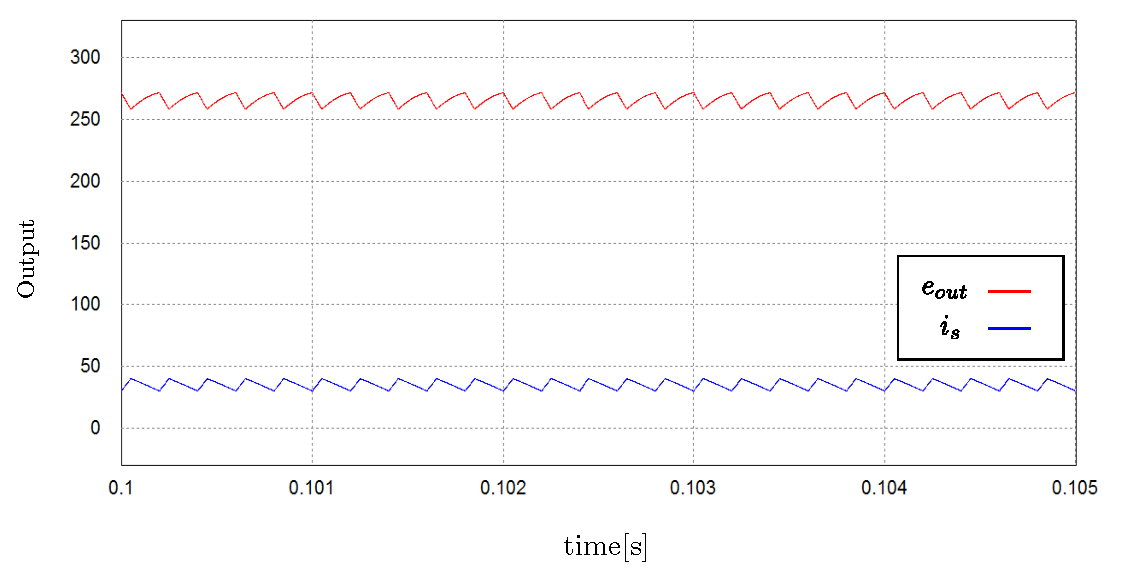
\includegraphics[scale=0.75]{../figure/eps/25.eps}\\
 (a) $ \alpha = 0.25 $ \\
 \vspace{0.3cm}
 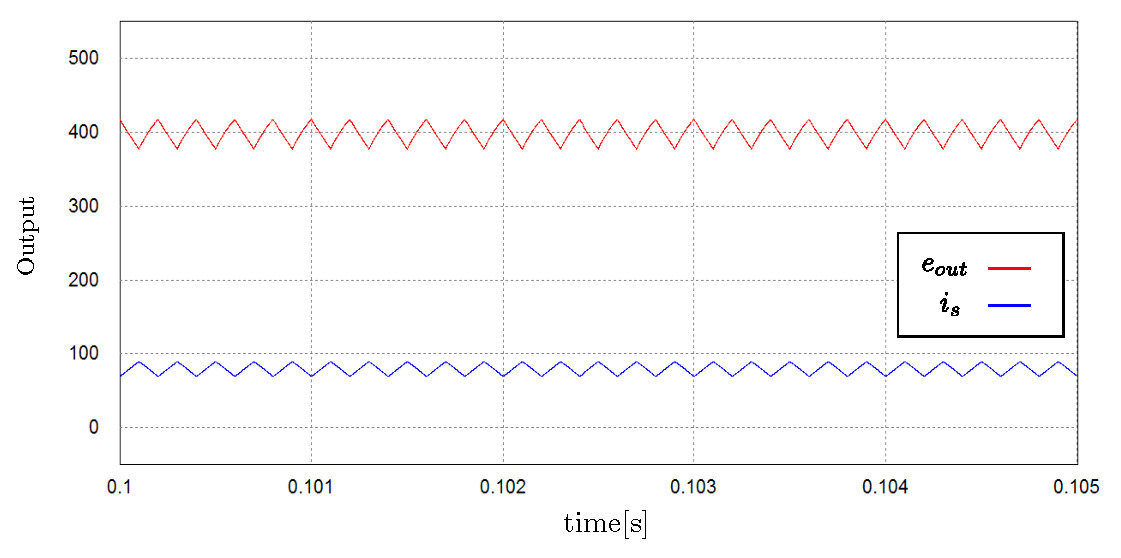
\includegraphics[scale=0.75]{../figure/eps/50.eps}\\
 (b) $ \alpha = 0.50 $ \\
 \vspace{0.3cm}
 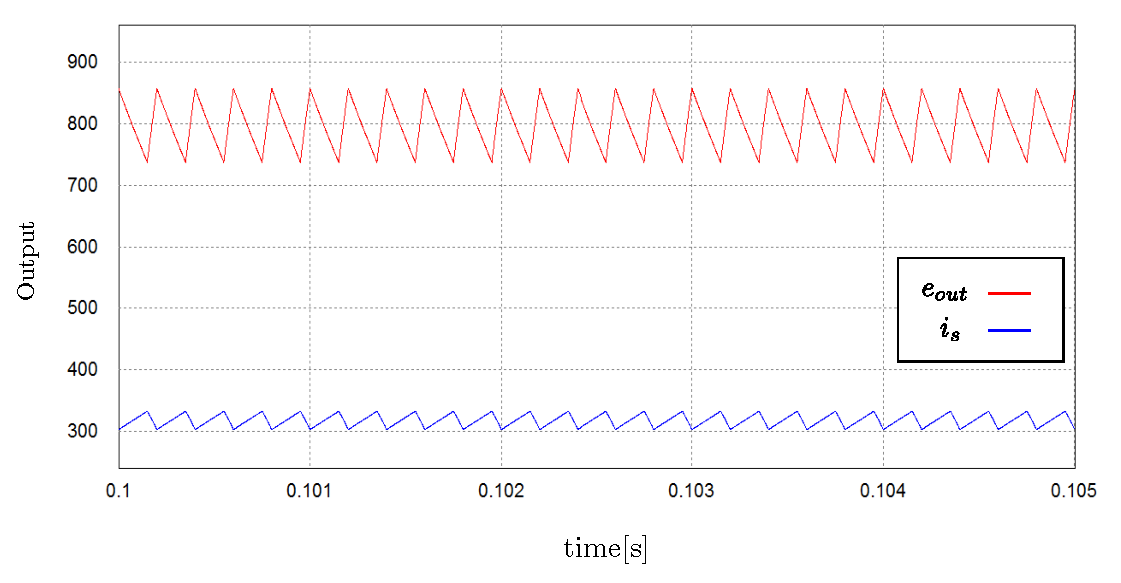
\includegraphics[scale=0.75]{../figure/eps/75.eps}\\
 (c) $ \alpha = 0.75 $ \\
 \caption{シミュレーション結果}
\label{result}
\end{figure}
%
%



% % 図の挿入

% \begin{figure}[b]
%  \begin{center}
%   \includegraphics[scale=0.9]{../figure/circuit.eps}
%   \caption{Uncontrolled converter}
%   \label{circuit}
%  \end{center}
% \end{figure}


% % 表の挿入

% \begin{table}[htb]
%   \begin{center}
%     \caption{各素子のパラメータ}
%     \begin{tabular}{c|c|c} \hline
%       定数名[単位] & 記号 & 値 \\ \hline \hline
%       周波数[Hz] & $f_U,f_V,f_W$ & 120 \\ \hline
%                      & $\phi_U$ & $\frac{2\pi}{3}$ \\
%       初期位相角[rad] & $\phi_V$ & $\frac{4\pi}{3}$ \\
%                      & $\phi_W$ & $2\pi$ \\ \hline
%       抵抗[$\Omega$] & $R$ & 10 \\ \hline
%     \end{tabular}
%     \label{param}
%   \end{center}
% \end{table}


% % 図の挿入

% \begin{figure}[tb]
%  \centering
%  \vspace{0.5cm}
%  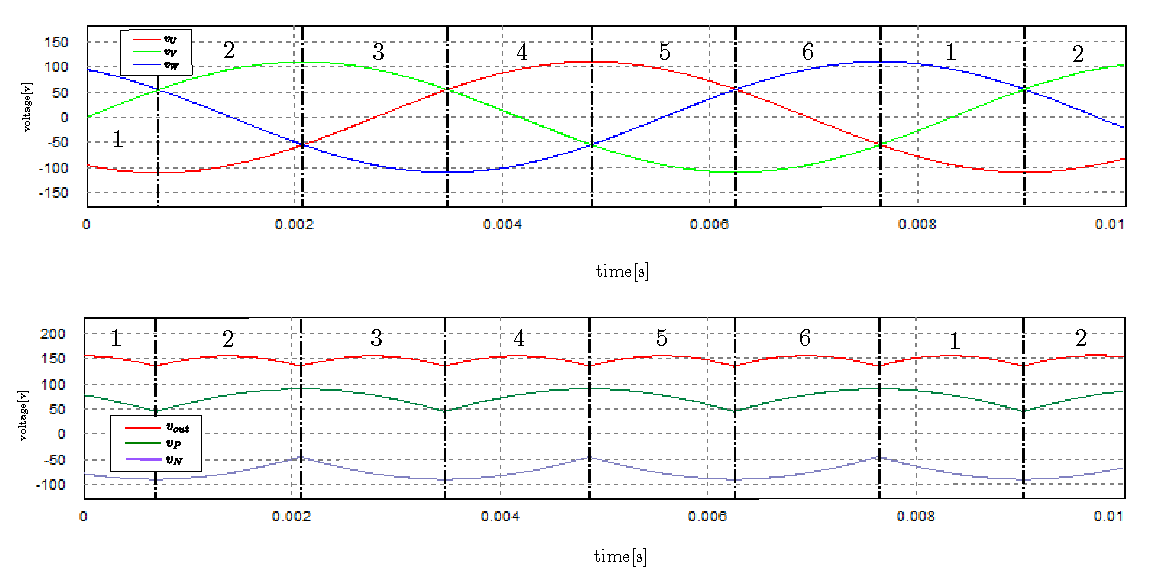
\includegraphics[scale=0.85]{../figure/waves.eps}\\
%  \hspace{0.0cm}
%  % 入力と出力\\
%  % \\
%  % \vspace{1.2cm}
%  % 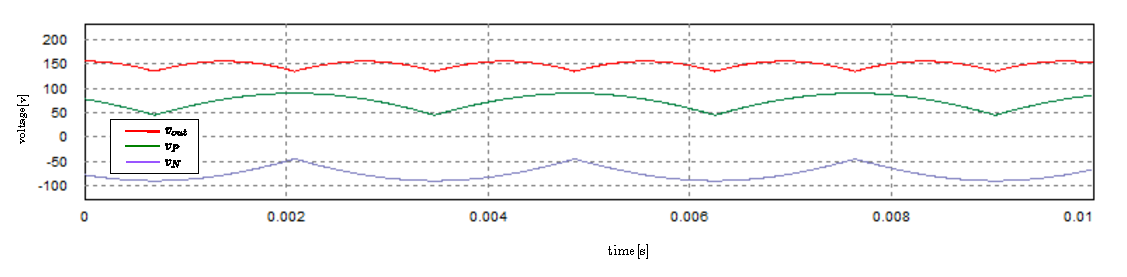
\includegraphics[scale=0.825]{../figure/output.eps}\\
%  % (b) 出力の電位\\
%  % \\
%  \caption{シミュレーションにより得られた各電源電圧(上)と出力電位(下)の波形}
%  \label{wave}
% \end{figure}

% \newpage

% % 図を並べて挿入

% \begin{figure}[tb]
%  \centering
%  \subfloat[区間1における回路動作]{\includegraphics[scale=0.5]{../figure/kukan_1.eps}}
%  \hspace{1.5cm}
%  \subfloat[区間2における回路動作]{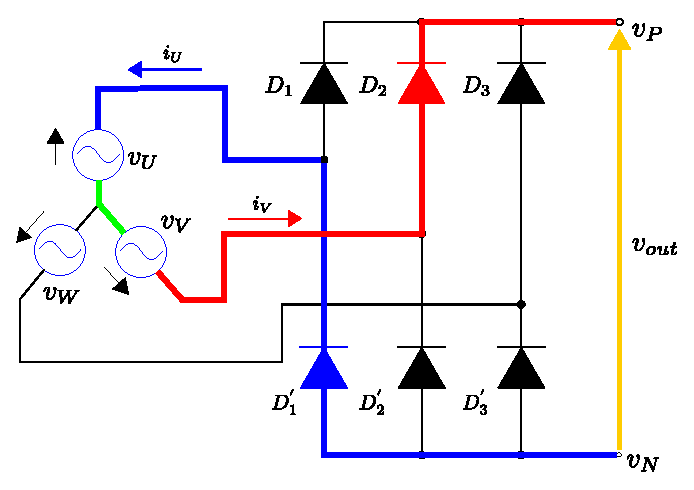
\includegraphics[scale=0.5]{../figure/kukan_2.eps}}
% \\
%  \vspace{0.5cm}
%  \subfloat[区間3における回路動作]{\includegraphics[scale=0.5]{../figure/kukan_3.eps}}
%  \hspace{1.5cm}
%  \subfloat[区間4における回路動作]{\includegraphics[scale=0.5]{../figure/kukan_4.eps}}
% \\
%  \vspace{0.5cm}
%  \subfloat[区間5における回路動作]{\includegraphics[scale=0.5]{../figure/kukan_5.eps}}
%  \hspace{1.5cm}
%  \subfloat[区間6における回路動作]{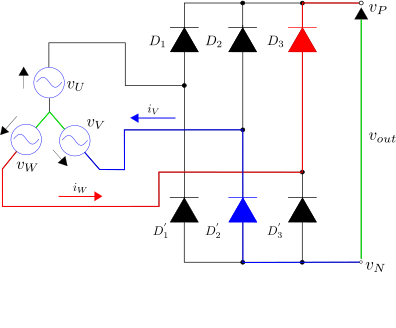
\includegraphics[scale=0.5]{../figure/kukan_6.eps}}
% \\
%  \caption{各区間での回路動作の様子}
%  \label{circuit_kaku}
% \end{figure}

% % 文中へのラベリング
% {\bf Fig. }\ref{circuit_kaku}に示す〜

% 参考文献
\begin{thebibliography}{99}
\addcontentsline{toc}{section}{参考文献}
\bibitem{1} 安部 可治,”パワーエレクトロニクスとシステム制御”,オーム社,pp.15-17,1991.
\bibitem{2} Atsuo Kawamura,”基礎パワーエレクトロニクス”,コロナ社,pp.88-90,1997.
\bibitem{3} 原田 耕介,”スイッチングコンバータの基礎”,コロナ社,pp.24-29,1993.
\bibitem{4} T.Sakamoto,”Lecture Note of Advanced Electrical Drive Control System”,pp.23,2017.
% \bibitem{3} 森本 雅之,”インバータ工学 -しくみから理解するインバータの技術-”,森北出版株式会社,pp.36-38,2011.
\end{thebibliography}

\end{document}
